\section{Results}
\label{sec:results}

\subsection{Reproduction}
\label{sec:res-repro}

Before changing anything we reproduced the published method from its released code on its own tasks. These tasks differ
from the rest of the paper in label space: the published Paderborn task has eight classes, each one physical bearing (K001,
KA04, KA15, KA22, KA30, KI14, KI17, KI21), so every target specimen is also a source specimen. On JNU the mean accuracy over
the six condition pairs is \SI{98.03}{\percent} against \SI{98.50}{\percent} reported; on Paderborn it is
\SI{96.20}{\percent} against \SI{96.78}{\percent}. The two hardest tasks bracket the published values over four seeds
(A3$\to$A2: $93.9\pm4.7$ against 97.84 reported; A1$\to$A2: $90.3\pm4.9$ against 87.03), and the seed standard deviation on
those tasks, about 5 points, exceeds many differences reported between competing methods in this literature. We treat the
method as reproduced and use the released hyper-parameters unchanged. Everything after this subsection uses the
three-class label space with several bearings per class; the leaky baselines below are measured in that space, not
against the published number.

\subsection{What survives bearing-disjoint evaluation}
\label{sec:res-collapse}

\begin{table}[htbp]
\centering
\caption{Paderborn: accuracy (\%) of SDALR (final checkpoint, seed 2024) on leaky and bearing-disjoint (clean) targets, the same gap for the source model before adaptation, and the clean target with the envelope threshold gate and with the oracle pseudo-label filter. Each entry is the mean over the six condition pairs of that split.}
\label{tab:collapse}
\small
\setlength{\tabcolsep}{4pt}
\begin{tabular}{lrrrrrrrr}
\toprule
Split & Leaky & Clean & $\Delta_{\mathrm{leak}}$ & Source-only $\Delta$ & Gated & Gain & Oracle & Recov.\ (\%) \\
\midrule
S00 & 91.5 & 66.5 & 25.0 & 34.8 & 69.7 & +3.1 & 89.0 & 90 \\
S01 & 96.1 & 39.8 & 56.3 & 50.6 & 62.5 & +22.6 & 95.1 & 98 \\
S02 & 88.8 & 51.6 & 37.2 & 35.4 & 60.9 & +9.3 & 73.9 & 60 \\
S03 & 93.8 & 58.6 & 35.2 & 29.3 & 57.2 & -1.5 & 75.5 & 48 \\
S04 & 82.2 & 74.0 & 8.2 & 2.0 & 77.6 & +3.6 & 92.1 & 222 \\
S05 & 98.0 & 36.4 & 61.6 & 64.3 & 45.4 & +9.0 & 85.1 & 79 \\
S06 & 90.2 & 68.6 & 21.6 & 21.2 & 73.3 & +4.7 & 83.3 & 68 \\
S07 & 99.2 & 51.5 & 47.8 & 41.1 & 52.1 & +0.7 & 91.9 & 85 \\
S08 & 97.1 & 37.6 & 59.4 & 55.0 & 60.0 & +22.3 & 91.1 & 90 \\
S09 & 89.5 & 60.1 & 29.4 & 24.4 & 64.4 & +4.3 & 82.5 & 76 \\
\midrule
fold A & 88.3 & 58.4 & 30.0 & 32.6 & 61.2 & +4.4 & 88.5 & -- \\
fold B & 99.9 & 55.3 & 44.6 & 45.8 & 62.3 & +7.0 & 76.8 & -- \\
\bottomrule
\end{tabular}
\begin{minipage}{\linewidth}\vspace{2pt}\footnotesize Medians over the ten random splits, with split-cluster bootstrap 95\,\% intervals: $\Delta_{\mathrm{leak}}$ 36.2~pp [25.0, 56.3] (range 8.2--61.6, 10/10, exact sign-flip $p = 0.001$); source-only $\Delta$, before any adaptation step, 35.1~pp [24.4, 50.6]; gate gain +4.5~pp [2.5, 15.7] (positive in 9/10, $p=0.003$); recoverable share 82\,\% [68, 94]. Below the rule, the two mechanical folds: leaky, clean and source-only columns from the fold job; gated and oracle from the gating job, with the gain taken against that job's own ungated clean arm (56.8 and 55.3\,\%). The two jobs trained different source checkpoints (Section~\ref{sec:protocol}) and the gating job has no leaky arm, so no recoverable share is given for the folds. A share above 100\,\% (S04) means the oracle arm beats the leaky arm. Differences are computed before rounding.\end{minipage}
\end{table}


\begin{figure}[htbp]
\centering
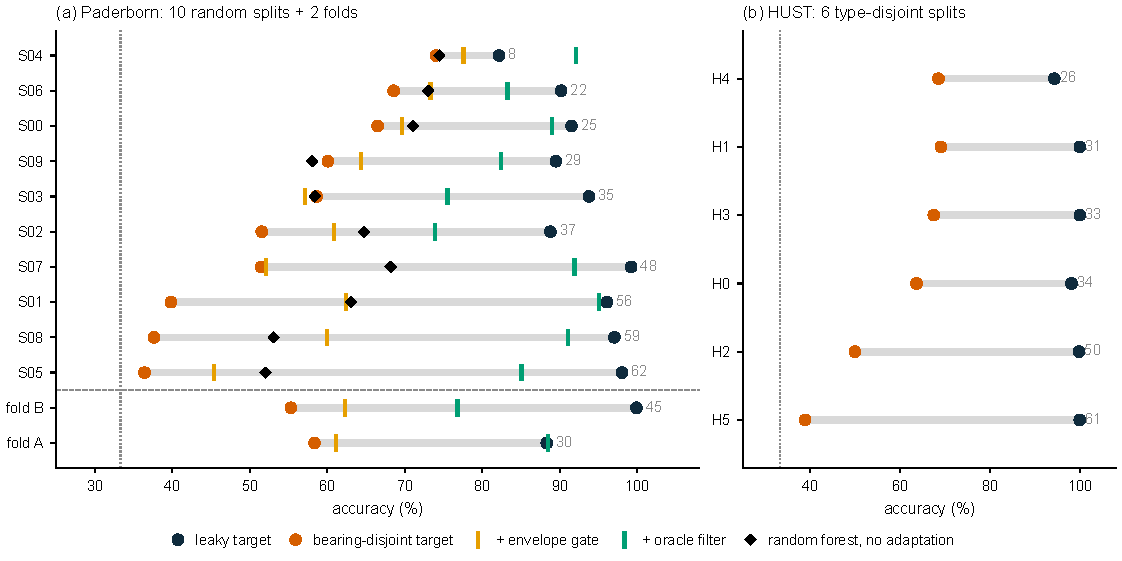
\includegraphics[width=\linewidth]{figures/fig2_collapse.pdf}
\caption{Accuracy by split on both rigs, rows sorted by the size of the collapse. Each row joins the leaky target (dark) to
the bearing-disjoint target (orange); ticks mark the same source model adapted with the envelope threshold gate (amber) and
with the oracle pseudo-label filter (green), and diamonds a random forest on ten time-domain statistics trained on the same
source windows without adaptation. The number at the right of each row is $\Delta_{\mathrm{leak}}$ in percentage points.
(a) Paderborn, ten pre-registered random bearing splits above the rule and the two mechanical folds below it (for the folds,
the ticks come from the gating job, whose source checkpoint differs from that of the dots; Section~\ref{sec:protocol});
(b) HUST bearing, six type-disjoint splits. Dotted line: three-class chance level.}
\label{fig:collapse}
\end{figure}

Across the ten pre-registered random splits (Table~\ref{tab:collapse}, Fig.~\ref{fig:collapse}) SDALR loses a median of 36.2
points on bearing-disjoint targets (95\,\% CI 25.0--56.3, range 8.2--61.6), positive in every split ($p=0.001$,
$p_{\mathrm{BH}}=0.002$). Which bearings happen to be in the source moves clean accuracy between \SI{36.4}{} and
\SI{74.0}{\percent}, which is why a single split --- the norm in this literature --- cannot support a performance claim. On
the two mechanical folds the leaky arm reaches \SI{94.1}{\percent} and the clean arm \SI{56.8}{\percent}, a loss of 30.0
points with fold~A as source and 44.6 with fold~B; with fold~B as source all six leaky tasks exceed \SI{99.7}{\percent} while
all six clean tasks fall between \SI{55.27}{} and \SI{55.33}{\percent}. The released checkpoint policy, which consults target
labels, gives \SI{94.7}{\percent} against \SI{57.8}{\percent} on the folds: target-label selection is worth 0.6 points on leaky
and 1.0 points on clean targets on average (per task 0.0--4.1), so it does not account for the gap.

\textbf{The gap is there before adaptation.} The batch-0 accuracy recorded in every adaptation log is the source model's
accuracy before any update. On the ten splits the source model alone already loses a median 35.1 points on unseen bearings
(CI 24.4--50.6, 10 of 10; Table~\ref{tab:collapse}, column ``Source-only $\Delta$''). SDALR's adaptation then changes the gap
by a median $+4.7$ points (positive in 8 of 10, two-sided $p = 0.18$): it raises leaky accuracy by a median 2.0 points and
lowers clean accuracy in 7 of 10 splits (median $-2.3$). On the folds adaptation adds 3.4 and 2.2 points on clean targets,
which is why an earlier reading of the folds alone suggested that adaptation helps there. Adaptation neither creates the
gap nor repairs it; the paper's subject is therefore what source-free adaptation inherits from its source model.

\textbf{The same bearing, seen and unseen.} Leaky and clean targets hold different bearings, so $\Delta_{\mathrm{leak}}$ also
contains the difference in difficulty between two bearing sets. Across the ten splits every bearing is in the source in some
splits and in the clean target in others, so its accuracy when seen can be compared with its accuracy when unseen
(Table~\ref{tab:bearings}, Fig.~\ref{fig:bearings}a). The within-bearing difference has a median of 38.7 points over the 17
bearings (CI 9.5--62.5): positive for 14 and tied for 3 (the healthy K003, K004 and K006, recognised perfectly either way); none is
negative. By class the median is 2.9 points for healthy specimens, 62.5 for outer-race and 49.0 for inner-race ones. Two
outer-race bearings, KA16 and KA30, are never correctly classified by SDALR when unseen. The seen and unseen scores come from
different adaptation runs and bearings share splits, so this contrast is descriptive; it holds the specimen fixed, which
the leaky--clean contrast cannot.

\subsection{The loss is not specific to one method, rig or condition shift}
\label{sec:res-second}

\begin{table}[htbp]
\centering
\caption{The collapse is not specific to one method: two source-free methods and four non-adaptive random forests on Paderborn, leaky versus bearing-disjoint targets (accuracy, \%).}
\label{tab:methods}
\begin{tabular}{lrrr}
\toprule
Method & Leaky & Clean & $\Delta_{\mathrm{leak}}$ \\
\midrule
SDALR, as released (target-label checkpoint) & 94.7 & 57.8 & 36.9 \\
SDALR, final checkpoint & 94.1 & 56.8 & 37.3 \\
SHOT, final iterate & 87.2 & 65.1 & 22.1 \\
\midrule
Random forest, 10 time statistics & 88.8 & 63.6 & 25.2 \\
Random forest, 64 spectral bands & 93.2 & 52.6 & 40.6 \\
Random forest, envelope spectrum & 76.7 & 43.1 & 33.5 \\
Random forest, all three feature sets & 95.4 & 60.3 & 35.1 \\
\midrule
Source model only (before adaptation), ten splits & 90.5 & 54.7 & 35.8 \\
Random forest, 10 time statistics, ten splits & 87.0 & 63.6 & 23.4 \\
Random forest, all three feature sets, ten splits & 93.1 & 57.6 & 35.5 \\
Random forest, 13 kinematic envelope features, ten splits & 67.4 & 54.3 & 13.1 \\
SHOT, final iterate, 10 splits & 82.7 & 57.4 & 25.3 \\
\bottomrule
\end{tabular}
\begin{minipage}{\linewidth}\vspace{2pt}\footnotesize All rows above the second rule use the same windows, the same two mechanical folds and the same 12 paired tasks; the random forests use no adaptation and no target data. No $p$-value is quoted for them: the tasks of a fold share a source checkpoint, so the unit is the fold, and two clusters cannot reach below $p = 0.25$ (Section~\ref{sec:protocol}). The rows below the second rule are means over the ten pre-registered splits, where the split is the unit; the time-statistics and combined forests collapse in 10 of 10 splits (exact sign-flip $p = 0.001$, $p_{\mathrm{BH}} = 0.002$). Source model only: batch-0 accuracy of the SDALR/SHOT source checkpoint before any adaptation step (median $\Delta$ 35.1~pp). Kinematic forest: record-level, maxima of the normalised envelope spectrum at the specimen's own BPFO/BPFI harmonics and shaft orders (median $\Delta_{\mathrm{leak}}$ 8.4~pp). SHOT over 10 splits: median $\Delta_{\mathrm{leak}}$ 21.7~pp, positive in 10 of 10 (exact sign-flip $p = 0.001$, $p_{\mathrm{BH}} = 0.002$). Differences are computed before rounding.\end{minipage}
\end{table}


\begin{table}[htbp]
\centering
\caption{Second rig: SDALR on HUST bearing, six pre-registered type-disjoint splits (accuracy, \%). The source is three bearing types; the clean target is the other two at the target load.}
\label{tab:hust}
\begin{tabular}{llrrr}
\toprule
Split & Source bearings & Leaky & Clean & $\Delta_{\mathrm{leak}}$ \\
\midrule
H0 & 6204, 6207, 6208 & 98.1 & 63.7 & 34.5 \\
H1 & 6204, 6205, 6207 & 100.0 & 69.1 & 30.9 \\
H2 & 6204, 6205, 6206 & 99.8 & 49.9 & 49.9 \\
H3 & 6205, 6206, 6207 & 100.0 & 67.5 & 32.5 \\
H4 & 6206, 6207, 6208 & 94.3 & 68.5 & 25.8 \\
H5 & 6205, 6206, 6208 & 100.0 & 38.9 & 61.1 \\
\bottomrule
\end{tabular}
\begin{minipage}{\linewidth}\vspace{2pt}\footnotesize Median $\Delta_{\mathrm{leak}}$ 33.5~pp (range 25.8--61.1, one-sided Wilcoxon $p=0.016$ over the six splits, which is the smallest value attainable with six clusters; exact sign-flip $p=0.016$, $p_{\mathrm{BH}}=0.022$, but $p_{\mathrm{BY}}=0.065$ under arbitrary dependence), which meets the replication rule fixed before the run. On this rig the clean target changes bearing size as well as bearing identity, so the shift is stronger than Paderborn's.\end{minipage}
\end{table}


Table~\ref{tab:methods} repeats the design for a second source-free method and for non-adaptive baselines. SHOT, in our
implementation and from the same source checkpoint, loses 22.1 points on the folds and a median of 21.7 over the ten splits
(CI 10.9--37.7, 10 of 10, $p = 0.001$, $p_{\mathrm{BH}} = 0.002$; the pre-registered rule --- a median loss of at least 10
points at $p < 0.05$ --- is met). Its smaller loss than SDALR's does not mean it transfers better: SHOT starts from the same
35.1-point source gap and narrows it mainly by lowering leaky accuracy (median $-5.3$ points) rather than by raising clean
accuracy (median $+3.7$). Random forests \cite{pedregosa2011sklearn} trained on the same source windows with no adaptation at all lose a median 22.7
points on ten time-domain statistics (CI 16.4--32.5) and 32.1 points on the combined feature set (CI 25.5--43.3), each in 10
of 10 splits ($p_{\mathrm{BH}} = 0.002$ each). On bearing-disjoint targets the time-statistics forest is more accurate than
adapted SDALR by a median 8.9 points (CI 0.4--16.1, 8 of 10 splits).

The result replicates on a second rig. On HUST bearing (Table~\ref{tab:hust}, Fig.~\ref{fig:collapse}b) mean leaky accuracy
is \SI{98.7}{\percent} and mean clean accuracy \SI{59.6}{\percent}, a median split-level loss of 33.5 points (CI 28.4--55.5,
$p=0.016$), meeting the replication rule fixed before the run. Each HUST bearing type is a different size, so the clean target
changes geometry as well as specimen, and with six clusters the result survives Benjamini--Hochberg but not
Benjamini--Yekutieli; it replicates direction and size.

\textbf{Without any condition shift.} Every task above crosses operating conditions. In a pre-registered control the time-
statistics forest is trained, at each condition separately, on half of the source bearings' recordings and tested at the
\emph{same} condition on the held-out recordings of the same bearings and on recordings of the complementary bearings;
recordings never cross the split, which is the separation used by recording-level benchmarks \cite{knap2026leakagesafe} and
the repetition-wise split of Vieira et al.\ \cite{vieira2026}. Balanced accuracy falls by a median of 29.7 points (CI
18.7--40.5, 10 of 10, $p_{\mathrm{BH}} = 0.002$), from a median \SI{94}{\percent} on held-out recordings of seen bearings to
\SI{65}{\percent} on unseen ones. Unseen-bearing accuracy is comparable with and without a condition shift (median balanced accuracy
\SI{65}{\percent} here, mean accuracy \SI{63.6}{\percent} across conditions), so condition shift is not what the leaky--clean
difference mainly measures. A post-hoc breakdown by class
locates the loss: healthy recall barely moves (median 99.9 to \SI{98.2}{\percent}); inner-race recall, where every bearing
carries the same mechanism (fatigue pitting \cite{lessmeier2016}), falls by a median 28.5 points; outer-race recall, which
mixes pitting with plastic deformation from indentations, falls by 66 points, and on unseen indentation bearings it is a
median \SI{23}{\percent} against \SI{64}{\percent} on pitting ones (medians over the ten and eight target sets that contain such bearings, folds included). This
control uses a forest; SDALR and SHOT were not run at a fixed condition.

\subsection{Why unseen bearings fail}
\label{sec:res-mechanism}

\begin{table}[htbp]
\centering
\caption{Per-bearing view of the Paderborn real-damage specimens: what each one is, how SDALR scores it when it was and was not in the source, and how often the envelope gate certifies it.}
\label{tab:bearings}
\small
\setlength{\tabcolsep}{4pt}
\begin{tabular}{lllllrrrr}
\toprule
Bearing & Mfr. & Damage & Extent & Size (mm) & Seen & Unseen & Diff. & Gate \\
\midrule
KA04 & FAG & pitting & 1 & 2 $\times$ 3 & 87 & 25 & +62 & 41/60 \\
KA15 & FAG & indentation & 1 & $<$1 $\times$ $<$1 & 68 & 29 & +39 & 0/60 \\
KA16 & MTK & pitting & 2 & 2 $\times$ full & 75 & 0 & +75 & 40/60 \\
KA22 & IBU/IBB & pitting & 1 & $<$2 $\times$ 1 & 100 & 55 & +45 & 0/60 \\
KA30 & MTK & indentation & 1 & $<$1 $\times$ $<$1 & 94 & 0 & +94 & 1/60 \\
KI04 & MTK & pitting & 1 & 2 $\times$ 1 & 84 & 61 & +23 & 0/60 \\
KI14 & MTK & pitting & 1 & 1 $\times$ 1 & 87 & 43 & +44 & 0/60 \\
KI16 & FAG & pitting & 3 & 6 $\times$ full & 95 & 41 & +54 & 32/60 \\
KI17 & MTK & pitting & 1 & 1 $\times$ 2 & 96 & 21 & +75 & 0/60 \\
KI18 & MTK & pitting & 2 & 2.5 $\times$ full & 96 & 31 & +65 & 45/60 \\
KI21 & FAG & pitting & 1 & 1 $\times$ 2 & 100 & 74 & +26 & 0/60 \\
\midrule
K001--K006 & IBU & healthy & -- & -- & 100 & 95 & +5 & 1/360$^{b}$ \\
\bottomrule
\end{tabular}
\begin{minipage}{\linewidth}\vspace{2pt}\footnotesize Manufacturer (page~1), damage mode, extent class (1--3) and damage length $\times$ width in mm (page~2) are read from each bearing's own Paderborn datasheet; pitting = fatigue pitting, indentation = particle-caused plastic deformation. Seen / unseen: SDALR window accuracy (\%) on that bearing over the ten splits in which it was in the source (scored in the leaky arm) or in the clean target. Gate: correct fault verdicts of the envelope threshold rule at the three adaptation conditions. $^{b}$ False acceptances. Over all 17 bearings the within-bearing difference has median 38.7~pp (95\,\% CI 9.5--62.5): 14 positive, 3 ties, 0 negative.\end{minipage}
\end{table}


\begin{figure}[htbp]
\centering
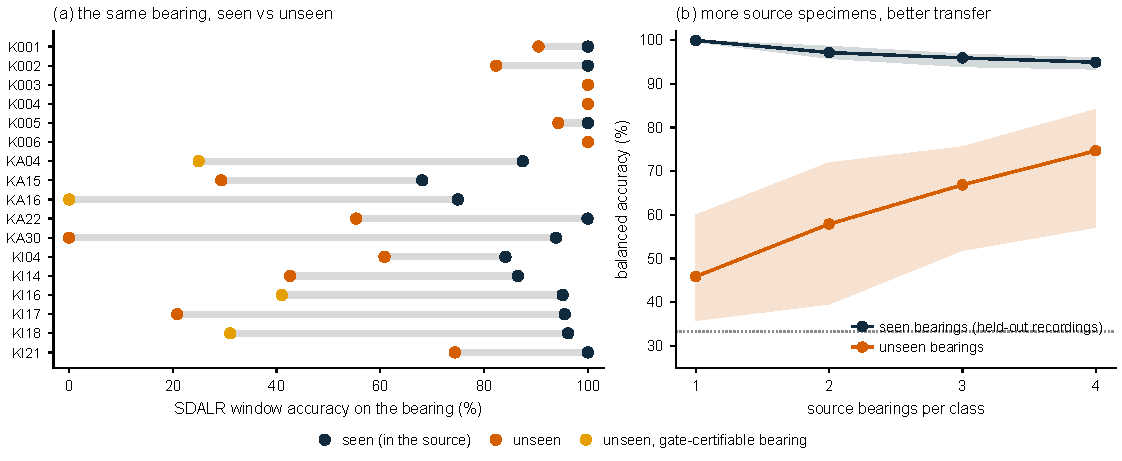
\includegraphics[width=\linewidth]{figures/fig3_bearings.pdf}
\caption{(a) SDALR accuracy on each Paderborn bearing over the ten splits, when it was in the source (dark) and when it was
unseen (orange; amber for the four bearings the envelope gate can certify). (b) Pre-registered source-diversity curve: a
random forest on ten time statistics, same-condition design, balanced accuracy on held-out recordings of the training
bearings (dark) and on one unseen bearing per class (orange), median and interquartile range over 30 test triples.}
\label{fig:bearings}
\end{figure}

Two explanations predict the same collapse. In one, a source-trained model learns to recognise its training specimens ---
a fixed identity shortcut --- and nothing about a new specimen. In the other, three specimens per class sample too little of
the variation in damage signatures (extent, shape, mechanism, manufacturer) for any classifier to cover a new one. The two
differ in what more source specimens would do, and in what a representation that encodes fault kinematics would do.

\textbf{Specimens are identifiable, but identifiability is not the failure.} A logistic-regression probe fitted within each
class on record-disjoint halves identifies the physical bearing in 507 of 508 held-out recordings from the frozen SDALR source
features and in 508 of 508 from ten elementary time statistics (pooled chance 0.35); the 508 recordings are the held-out half
of the 1020 source recordings of the six source models. The identification survives removing the signal mean, the statistic
most tied to sensor offset (508 of 508); the standard deviation alone identifies 477. It is not within-session drift: the
same probe asked to separate the first ten from the last ten recordings of one bearing succeeds on 285 of 508 (chance 254).
But healthy specimens are identified as perfectly as faulty ones (180 of 180) and still transfer (Table~\ref{tab:bearings}).
Identity is available in these signals; whether a classifier relies on it is a different question.

\textbf{More source specimens transfer better.} In a pre-registered curve the forest was trained on one to four source
bearings per class and tested on a fixed unseen bearing per class, for 30 test triples at each of the three conditions
(Fig.~\ref{fig:bearings}b). Balanced accuracy on the unseen bearings rises from a median \SI{45.9}{\percent} with one
specimen per class to 57.9, 66.9 and \SI{74.6}{\percent} with two, three and four, while accuracy on held-out recordings of
the training bearings stays at 95--100\,\%. The paired gain from one to four specimens has a median of 15.4 points over the
triples (25 of 30 positive, $p < 10^{-5}$), meeting the rule fixed before the run. A pure identity shortcut predicts a flat
curve; the measured one is steep. The collapse is therefore mainly under-sampling: with three specimens per class, the
source does not span the damage signatures it will meet, which is the supervised finding of Vieira et al.\ on the number of
training bearings \cite{vieira2026}, here measured as a curve under a fixed test set.

\textbf{Labelling whole specimens is not a sign of failure.} An adapted model that misclassifies an unseen bearing usually
does so for all its windows: with fold~B as source every clean bearing receives a single label across all six tasks, and the
resulting \SI{55.33}{\percent} is exact arithmetic (three healthy and two fault bearings right, $(2\,000 + 660 + 660)/6\,000$).
But block labelling is equally common when the bearing was seen: per task, \SI{90}{\percent} of seen and \SI{89}{\percent} of
unseen bearing--task pairs receive one label for at least \SI{99}{\percent} of their windows, and the fold~A direction is not
pure (K004 0.67, KI17 0.56). A specimen's windows are similar to each other, so a classifier decides the specimen as a whole;
the failure is in which label it gives, not in how it gives it.

\textbf{A kinematic representation leaks less but knows less.} The networks and forests above see 2048-sample windows,
which cannot represent the kinematic signature (Section~\ref{sec:windows}). A pre-registered forest on 13 kinematic features
of each full recording --- the floor-normalised envelope spectrum at the specimen's own first five outer- and inner-race
harmonics and at shaft orders 1--3 --- loses a median 8.4 points on unseen bearings (CI 4.8--21.0, 9 of 10 splits), below the
10-point threshold fixed in advance, so by its rule it transfers. Its accuracy is low on both arms (median \SI{65.8}{\percent}
leaky, \SI{56.1}{\percent} clean): the kinematic lines are visible only on the specimens with large damage (next subsection),
and a classifier that relies on them generalises as far as they are visible and no further. The representation decides how
much of what a model knows is specimen-specific; it does not by itself supply detectability. Concurrent work reports a
similar role for order-domain inputs in unsupervised adaptation across held-out Paderborn bearings, most of them with
artificial damage \cite{nagaswetha2026}.

\subsection{How much an oracle pseudo-label filter recovers}
\label{sec:res-decomp}

\begin{figure}[htbp]
\centering
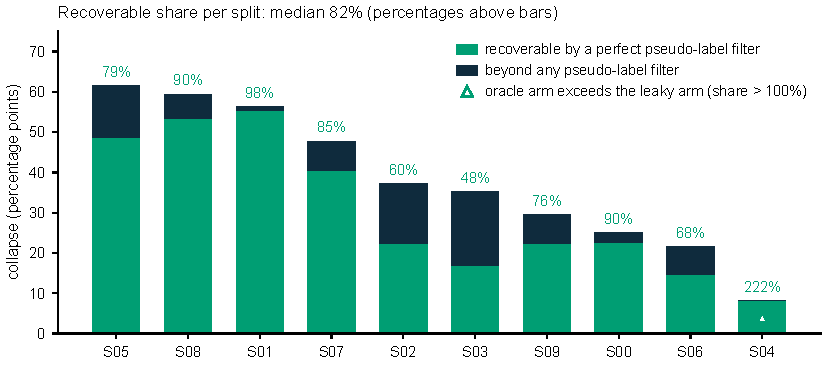
\includegraphics[width=\linewidth]{figures/fig4_decomposition.pdf}
\caption{Decomposition~\eqref{eq:decomp} per split: the part of the collapse an oracle pseudo-label filter recovers, and the
part it does not.}
\label{fig:decomp}
\end{figure}

On the ten random splits, where all four arms ran in one job, the oracle filter recovers a median \SI{82}{\percent} of the
collapse (CI 68--94, interquartile range 70--\SI{90}{\percent}, Fig.~\ref{fig:decomp}). The share varies: at
\SI{48}{\percent} on S03 half the collapse is not recovered, while on S04 --- the mildest collapse, 8.2 points --- the oracle
arm exceeds the leaky arm, a share of \SI{222}{\percent}. The fold-level decomposition is not reported, because the gating job
that produced the oracle arm has no leaky arm (Section~\ref{sec:protocol}).

The oracle withholds every incorrect pseudo-label and keeps every correct one; it is the keep-or-withhold counterpart of the
perfect-pseudo-label level of Schlachter et al.\ \cite{schlachter2025}. It is a reference for filters acting on this
method's pseudo-label step --- the family to which all four gates belong --- not a proven bound, and it says nothing about
methods that relabel, reweight continuously or change the representation. The part it does not recover mixes what the
source model carries with the difference in difficulty between the two bearing sets, as S04 shows. With that reading,
correct pseudo-labels alone would close most of the gap on this rig; the question for physics gating is how many of them it
can supply.

\subsection{Physics gating: safety, coverage and paired gains}
\label{sec:res-gating}

\begin{table}[htbp]
\centering
\caption{Gate safety on real healthy bearings. A false acceptance is a healthy recording given a fault verdict.}
\label{tab:gates}
\small
\setlength{\tabcolsep}{4pt}
\begin{tabular}{lrrrrr}
\toprule
Gate (swept parameter) & Op.\ point & Healthy FA & 95\,\% CI (\%) & Correct verdicts & At zero FA \\
\midrule
Envelope threshold rule (PCV-like), $z$ & 10 & 1/480 & 0.0--1.2 & 366 & 351 \\
Shaft-alias-guarded comb (comb\_v2), $\alpha$ & 0.05 & 0/480 & 0.0--0.8 & 312 & 312 \\
Surrogate-null comb test, $\alpha$ & 0.05 & 9/480 & 0.8--2.9 & 309 & -- \\
Raw-spectrum band rule (EAGLE-style), $z$ & 2 & 214/480 & 26.9--60.8 & 429 & 0 \\
\bottomrule
\end{tabular}
\begin{minipage}{\linewidth}\vspace{2pt}\footnotesize Population: 2{,}319 Paderborn recordings (480 healthy, 1{,}839 single inner- or outer-race). Operating points are the values fixed before the gates were evaluated. The last column sweeps each gate's parameter and reports the largest number of correct fault verdicts reachable while accepting no healthy recording. Intervals: bootstrap over the 6 healthy bearings where the count exceeds one, exact Clopper--Pearson over records otherwise. Full operating curves: Supplementary~S2. The population spans 29 physical bearings -- 6 healthy, 11 real-damage and 12 artificial-damage -- at all four operating conditions; coverage by damage origin is given in Section~\ref{sec:res-gating}.\end{minipage}
\end{table}


\begin{figure}[htbp]
\centering
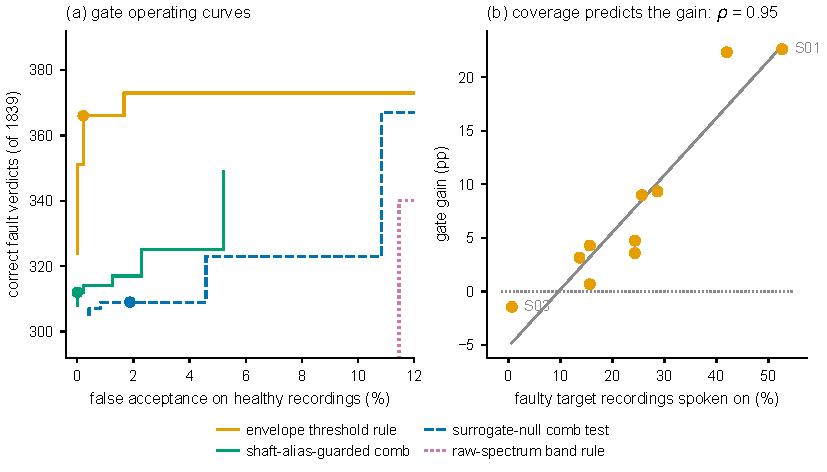
\includegraphics[width=\linewidth]{figures/fig5_roc.pdf}
\caption{(a) Gate operating curves on 2319 Paderborn recordings: correct fault verdicts against false acceptance on the 480
healthy recordings, as each gate's parameter is swept. Filled circles mark the operating points fixed before evaluation. The
vertical axis starts at 292 verdicts: the raw-spectrum band rule returns no correct verdict below \SI{11.5}{\percent} false
acceptance, and its operating point lies at \SI{45}{\percent}, off the right of the axis. (b) Per split ($n=10$), the share of
the clean target's faulty recordings the envelope gate gives a fault verdict against its paired accuracy gain. Spearman
$\rho = 0.95$; with the label-free share of all target recordings, $\rho = 0.93$. The line is a least-squares fit for reading
only.}
\label{fig:roc}
\end{figure}

\textbf{Safety.} Gate behaviour is characterised on all 2319 single-fault and healthy Paderborn recordings: 29 physical
bearings (6 healthy, 11 real-damage, 12 artificial-damage) at four operating conditions. At the operating points fixed
before evaluation (Table~\ref{tab:gates}) the envelope threshold rule accepts a fault on 1 of 480 healthy recordings (95\,\%
CI 0.0--1.2\,\%), the alias-guarded comb on none (0.0--0.8\,\%), the surrogate-null comb on 9 (0.8--2.9\,\%), and the
raw-spectrum band rule on 214 (26.9--60.8\,\%, bootstrapped over the six healthy bearings). Sweeping each gate's parameter
(Fig.~\ref{fig:roc}a) shows that this is not a threshold artefact: the envelope rule dominates at every false-acceptance
level and the raw-spectrum rule is dominated everywhere.

\textbf{Coverage, and what limits it.} No gate exceeds about \SI{20}{\percent} correct fault verdicts (the envelope rule's 373
of 1839) before false acceptance passes \SI{10}{\percent}. The comb tests, which add cepstral pre-whitening and a
record-specific null to the same kurtogram band selection, reach 323--349 below \SI{10}{\percent} false acceptance,
so the limit is not one detector's
design. Table~\ref{tab:bearings} shows where it lies. At the three adaptation conditions the envelope rule certifies 4 of the
11 real-damage bearings on more than one recording --- KA04 (41 of 60), KA16 (40), KI16 (32) and KI18 (45) --- and these are the
specimens with the largest damage: extent class 2 or 3, or a pit \SI{2}{mm} long and \SI{3}{mm} wide (KA04), with the damage
spanning the full raceway width on three of them. Every bearing it does not certify has extent class 1 and damage no larger
than \SI{2}{mm} in either dimension. The two comb tests certify the same four bearings (both also fire on a few recordings of
KI04, all wrongly, and of KA30); the raw-spectrum rule fires on every recording of those four, but also on bearings with no
envelope signature and on healthy ones. On this rig, envelope detectability is a
property of damage size, and a gate can only supply labels for the specimens whose damage is large enough to be seen.

\textbf{Inside the adaptation loop.} Over the ten splits the envelope gate adds a median 4.5 points to bearing-disjoint
accuracy (CI 2.5--15.7, positive in 9 of 10, $p=0.003$, $p_{\mathrm{BH}}=0.005$) and closes a median \SI{19}{\percent} of the
oracle gap (CI 10--41). Where it acts it changes what the model says --- with fold~B as source, KA04 moves from
\SI{100}{\percent} inner-race predictions to 71/29 inner/outer --- but the gain lies almost entirely on the recordings it
certifies (Table~\ref{tab:gateacc}). Splitting each split's clean windows by gate verdict, certified windows gain a median 47 points, uncovered faulty
windows a median 0.3 (sum over splits slightly negative) and healthy windows a median 0; certified windows carry
\SI{104}{\percent} of the summed gain. Because SFDA is scored on the windows it adapts on, a gain on certified windows is
partly the gate's own label returned. The size of the gain therefore follows coverage closely: across the splits it tracks
the share of faulty target recordings the gate speaks on ($\rho = 0.95$) and the label-free share of all target recordings
it speaks on ($\rho = 0.93$, $p = 10^{-4}$), and the latter survives partialling out headroom (oracle minus ungated clean;
partial $\rho = 0.90$, $p = 9\times10^{-4}$), whereas headroom given faulty-recording coverage predicts nothing (partial $\rho = 0.04$). The
coverage of a split is set by whether KA04, KA16, KI16 or KI18 are among its clean bearings. On S03, where the gate speaks
on two recordings of KA30 and is right on one, gating costs 1.5 points.

On the two mechanical folds, over three seeds, the alias-guarded comb adds a mean $+4.03$ points and the envelope rule
$+7.05$, positive in every seed (Table~\ref{tab:gains}, Fig.~\ref{fig:gains}); the comb was never run on the splits and no
general claim is made for it. The raw-spectrum band rule, run on the folds with one seed only, has a mean effect of $-3.9$
points that hides $+5.4$ with fold~A as source and $-13.2$ with fold~B: it injects confident wrong labels on healthy and
uncertified bearings, and whether that helps or hurts depends on which bearings are in the target.

\begin{table}[htbp]
\centering
\caption{Where the envelope-gate gain comes from: clean-target accuracy (\%) on certified and silent recordings.}
\label{tab:gateacc}
\small
\setlength{\tabcolsep}{4pt}
\begin{tabular}{lrrrrrrr}
\toprule
Split & Cert.\ (\%) & Certified & Silent faulty & Silent healthy & Gain & from cert. & from silent \\
\midrule
S00 & 12 & 51.2 $\to$ 99.2 & 59.5 $\to$ 55.2 & 83.5 $\to$ 83.5 & +3.1 & +5.6 & -2.4 \\
S01 & 37 & 10.1 $\to$ 70.3 & 9.3 $\to$ 11.2 & 100.0 $\to$ 100.0 & +22.6 & +22.0 & +0.6 \\
S02 & 20 & 29.8 $\to$ 75.8 & 26.3 $\to$ 27.0 & 100.0 $\to$ 100.0 & +9.3 & +9.0 & +0.3 \\
S03 & 1 & 0.0 $\to$ 0.5 & 38.4 $\to$ 36.2 & 99.7 $\to$ 99.7 & -1.5 & +0.0 & -1.5 \\
S04 & 17 & 50.5 $\to$ 71.0 & 64.8 $\to$ 64.8 & 100.0 $\to$ 100.0 & +3.6 & +3.6 & +0.0 \\
S05 & 14 & 4.3 $\to$ 55.7 & 22.8 $\to$ 22.8 & 71.9 $\to$ 76.7 & +9.0 & +7.3 & +1.6 \\
S06 & 17 & 49.2 $\to$ 74.1 & 54.1 $\to$ 55.0 & 100.0 $\to$ 100.0 & +4.7 & +4.3 & +0.4 \\
S07 & 9 & 38.6 $\to$ 55.8 & 29.5 $\to$ 30.6 & 93.3 $\to$ 88.7 & +0.7 & +1.5 & -0.9 \\
S08 & 31 & 10.0 $\to$ 80.4 & 3.5 $\to$ 5.3 & 100.0 $\to$ 100.0 & +22.3 & +21.7 & +0.7 \\
S09 & 9 & 7.4 $\to$ 76.6 & 45.1 $\to$ 42.0 & 100.0 $\to$ 100.0 & +4.3 & +6.1 & -1.8 \\
\bottomrule
\end{tabular}
\begin{minipage}{\linewidth}\vspace{2pt}\footnotesize Clean target of each split, SDALR ungated $\to$ with the envelope threshold gate, windows grouped by the gate verdict of their recording. Certified: a fault verdict; silent faulty and silent healthy: no verdict. The split's gain is the sum of the last two columns (group share $\times$ within-group change). Over the ten splits, certified windows gain a median 47~pp, silent faulty windows +0.3~pp; certified windows carry 104\,\% of the summed gain. SFDA is scored on the windows it adapts on, so the certified column partly returns the gate's own labels (C107).\end{minipage}
\end{table}


\begin{table}[htbp]
\centering
\caption{Paired per-task effect of gating inside SDALR on the 12 bearing-disjoint tasks of the two mechanical folds (gated $-$ ungated, percentage points).}
\label{tab:gains}
\small
\setlength{\tabcolsep}{4pt}
\begin{tabular}{llrrrrr}
\toprule
Gate & Seed & Mean & Median & Min & Max & Tasks $>0$ \\
\midrule
Shaft-alias-guarded comb & 0 & +3.79 & +3.33 & -0.08 & +11.01 & 7/12 \\
 & 1 & +4.56 & +3.28 & -0.08 & +15.45 & 8/12 \\
 & 2024 & +3.73 & +3.67 & -0.05 & +8.07 & 8/12 \\
\midrule
Envelope threshold rule & 0 & +7.44 & +7.57 & -0.01 & +18.02 & 9/12 \\
 & 1 & +7.99 & +6.65 & -0.70 & +19.44 & 10/12 \\
 & 2024 & +5.70 & +5.59 & -0.05 & +14.52 & 10/12 \\
\midrule
Raw-spectrum band rule & 2024 & -3.93 & -4.03 & -20.01 & +6.63 & 6/12 \\
\bottomrule
\end{tabular}
\begin{minipage}{\linewidth}\vspace{2pt}\footnotesize Every arm of a comparison runs in one job on the same source checkpoint, verified from identical pre-update target accuracy in each adaptation log, so these are paired differences. The between-seed spread of the per-task gain is 1.7~pp (comb) and 2.4~pp (envelope), against 2.8~pp for ungated per-task accuracy. No $p$-value is quoted: the 12 tasks of a seed come from two source folds, so the unit is the fold and two clusters cannot reach below $p = 0.25$. The inferential test is the ten-split comparison in Table~\ref{tab:collapse}. Raw-spectrum band rule: seed 2024 only and never run on the ten splits; its fold means are +5.35 (fold A source) and -13.21~pp (fold B source).\end{minipage}
\end{table}


\begin{figure}[htbp]
\centering
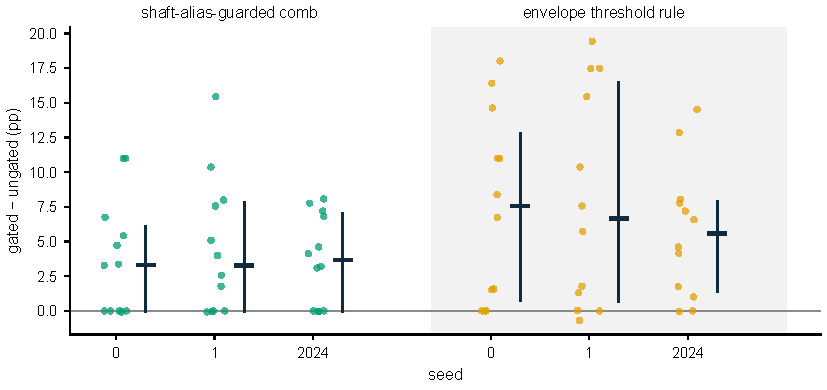
\includegraphics[width=\linewidth]{figures/fig6_gains.pdf}
\caption{Paired per-task effect of inserting each safe gate into the adaptation loop on the two folds, over three seeds.
Each point is one task; positive values are gains over the ungated arm trained from the same source checkpoint in the same
job. Horizontal mark: median; vertical bar: percentile bootstrap interval of the median over the 12 tasks (descriptive; tasks
of a fold share a checkpoint).}
\label{fig:gains}
\end{figure}

\textbf{Does the operating point need the target rig?} Gate verdicts use no target labels, but the evidence that $z = 10$ is
\emph{safe} comes from Paderborn's own healthy recordings, which is target-rig supervision. Swept on 24 healthy recordings
from two rigs that appear nowhere in the adaptation experiments --- 20 from UORED and 4 CWRU baselines, truncated to
Paderborn's spectral resolution --- the same rule needs $z = 36$ for zero false acceptance and accepts 4 of the 24 at $z = 10$.
On Paderborn the nearest swept point, $z = 40$, certifies 333 of 1839 fault recordings against 366 at $z = 10$
(\SI{91}{\percent} of the verdicts) with no healthy false acceptance. An operating point does not transfer between rigs and must be characterised on healthy recordings wherever the
gate is deployed; the adaptation arms were run at $z = 10$ only.
